\section{MTurk 截图} \label{sec:mturk}


\iffalse

\begin{figure}[h!]
    \centering
    \includegraphics[width=0.\linewidth]{imgs/}
    \caption{}
    \label{fig:}
\end{figure}


\fi

\begin{figure}[h!]
    \centering
    
\includegraphics[width=0.7\linewidth]{imgs/mturk/home.png}
    \caption{主页}
    \label{fig:home}
\end{figure}

\newpage

\begin{figure}[h!]
    \centering
    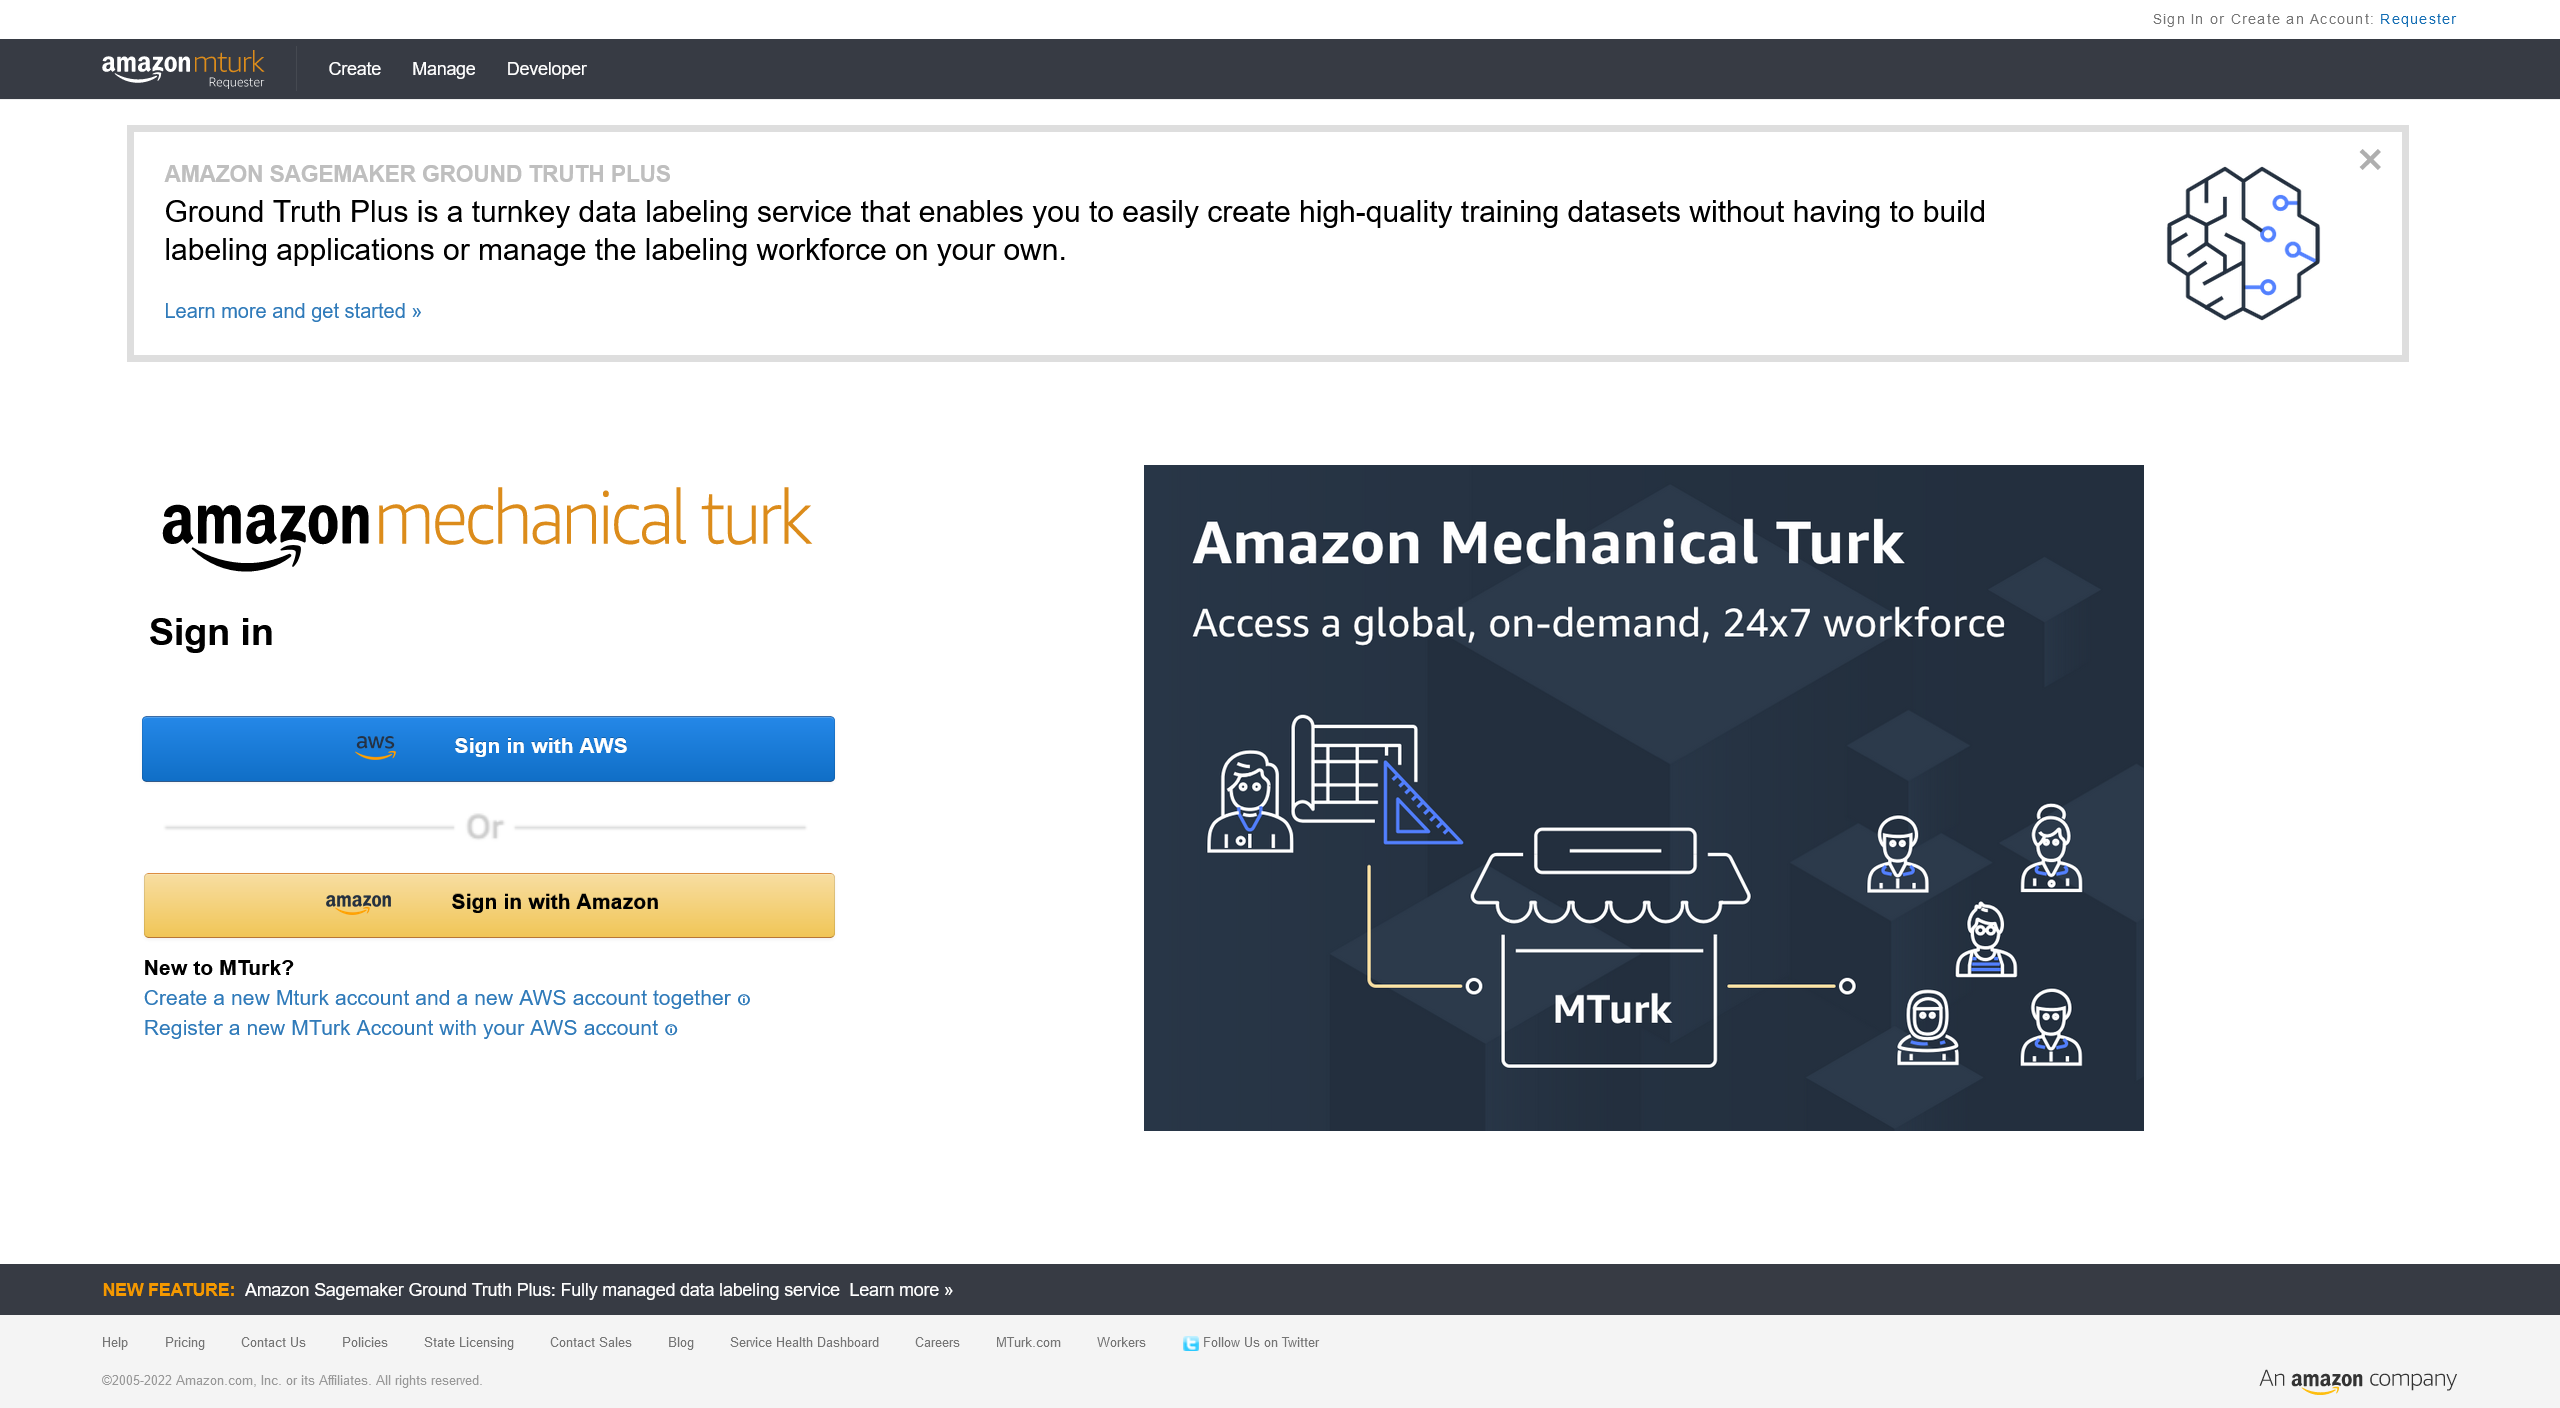
\includegraphics[width=0.9\linewidth]{imgs/mturk/login.png}
    \caption{登录}
    \label{fig:login}
\end{figure}

\begin{figure}[h!]
    \centering
    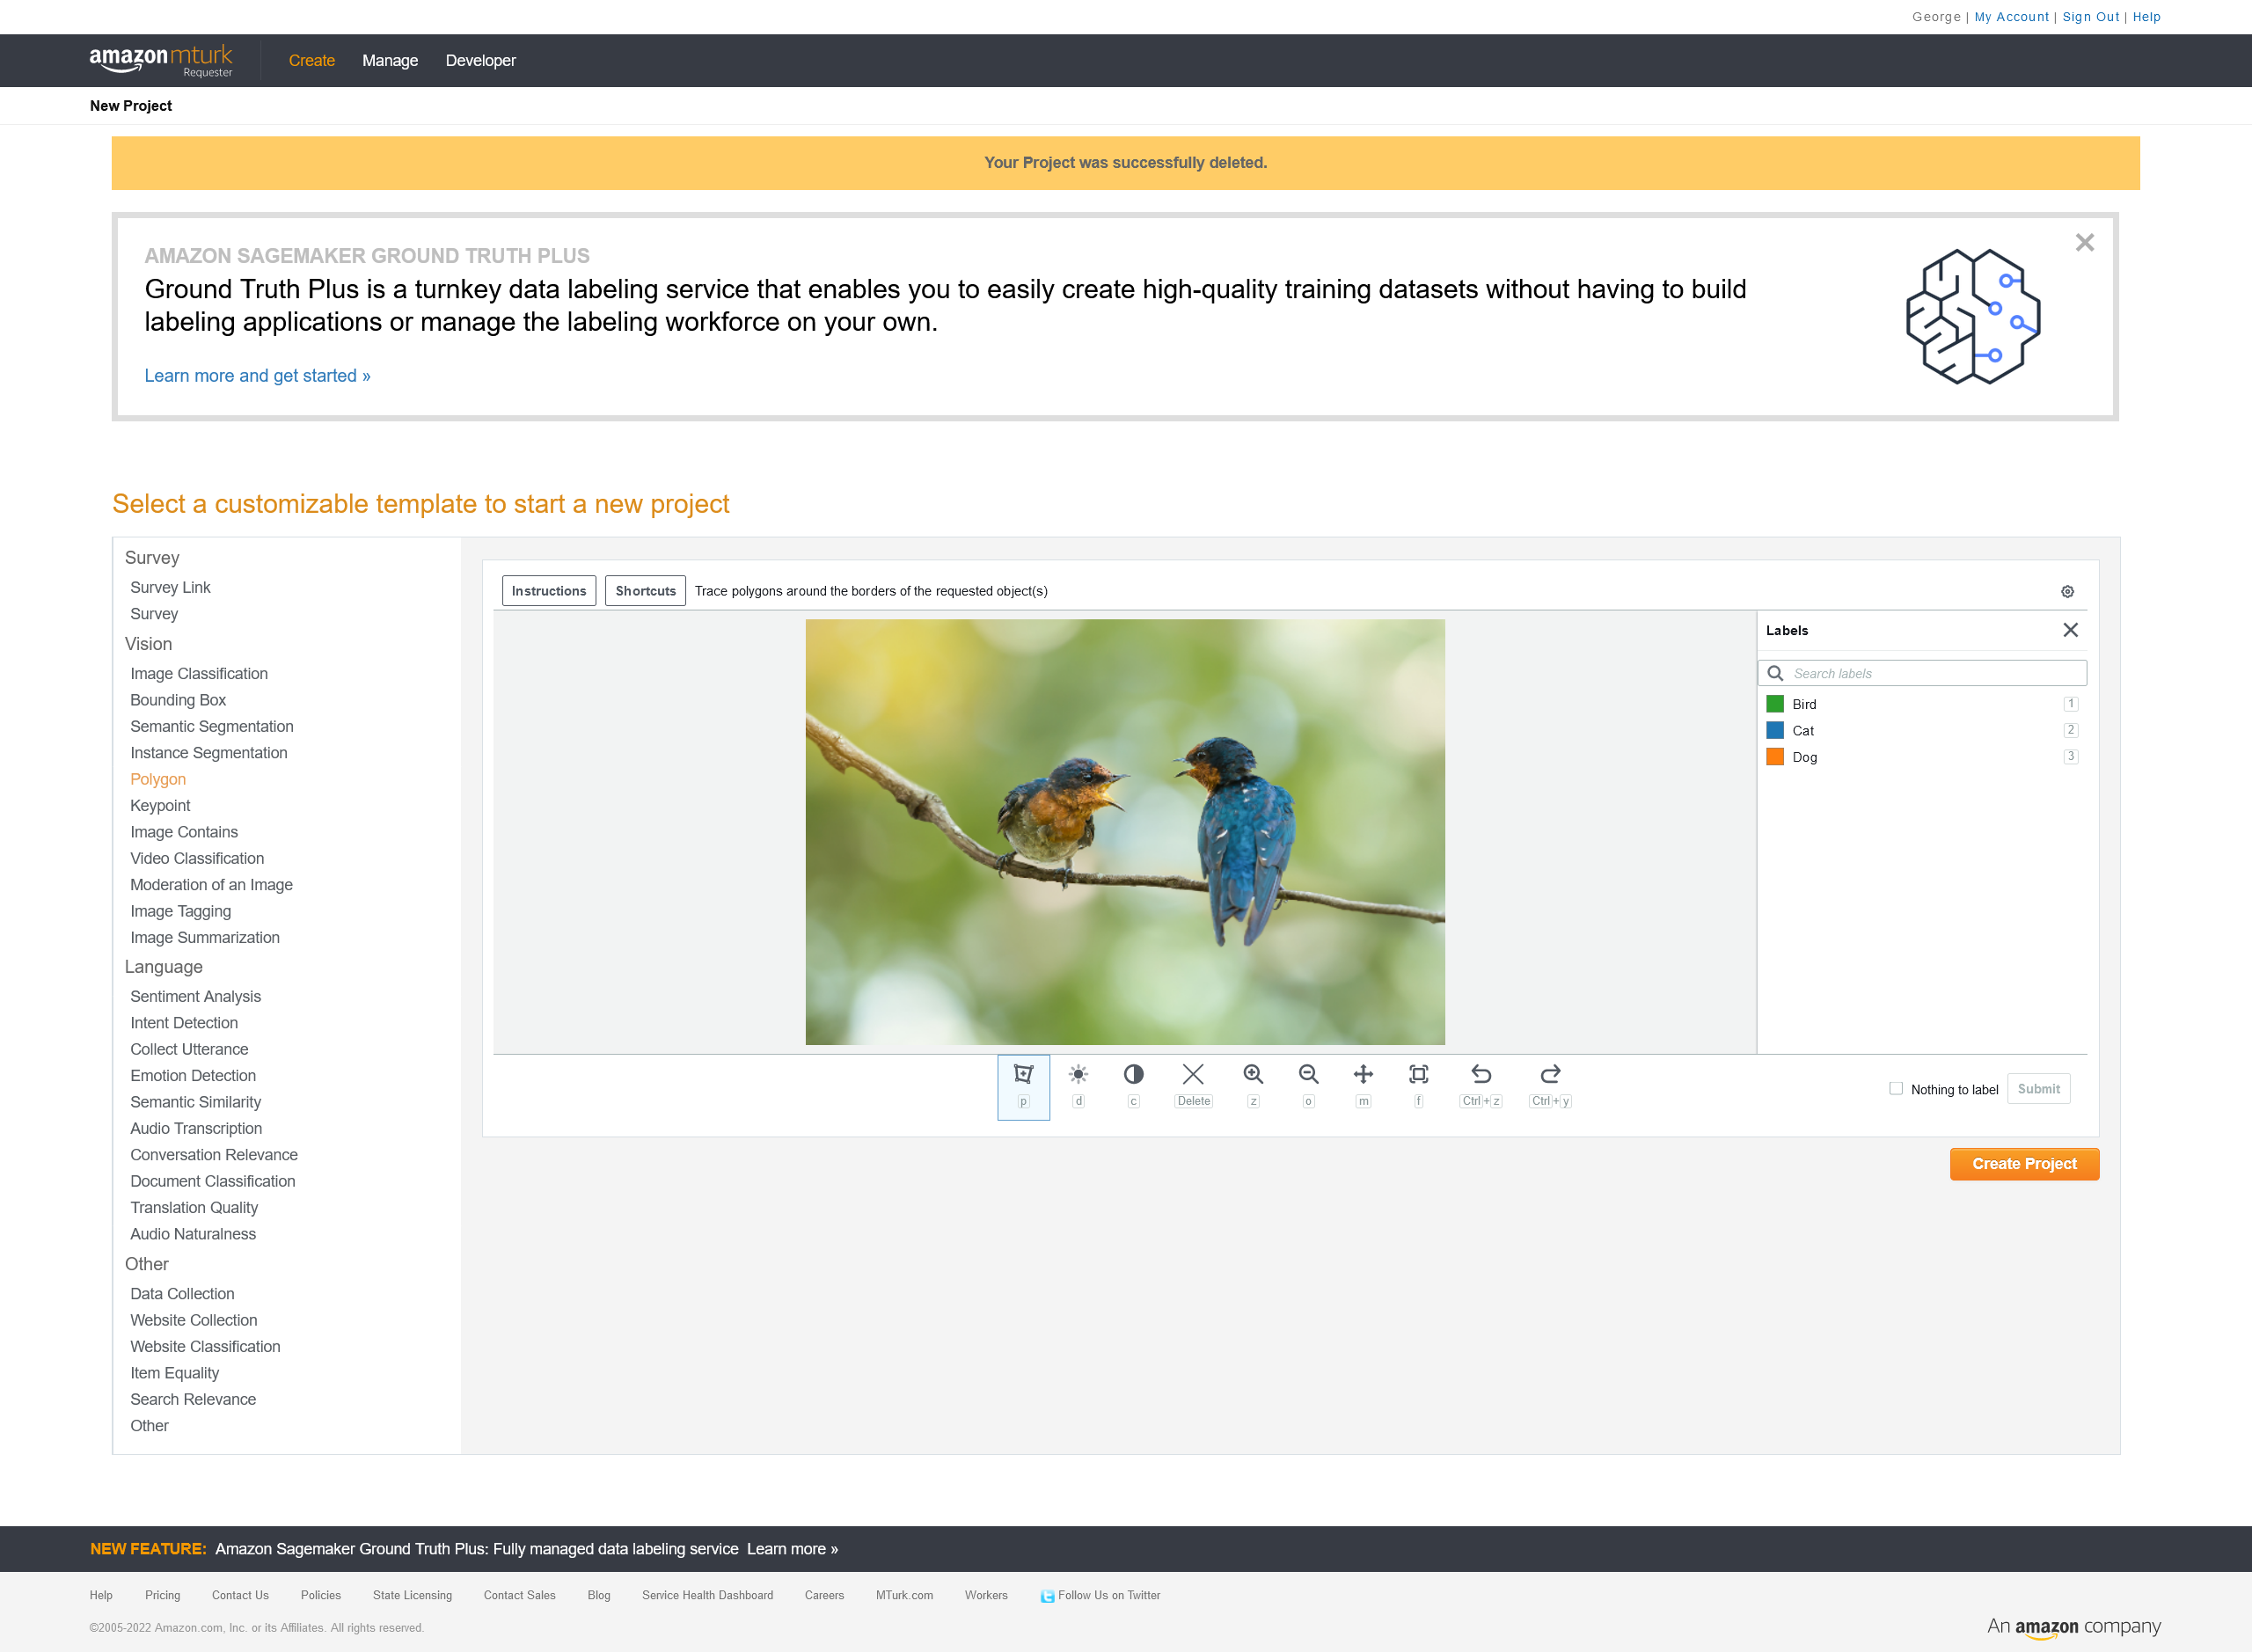
\includegraphics[width=0.9\linewidth]{imgs/mturk/template.png}
    \caption{任务模板}
    \label{fig:template}
\end{figure}

\newpage

\begin{figure}[h!]
    \centering
    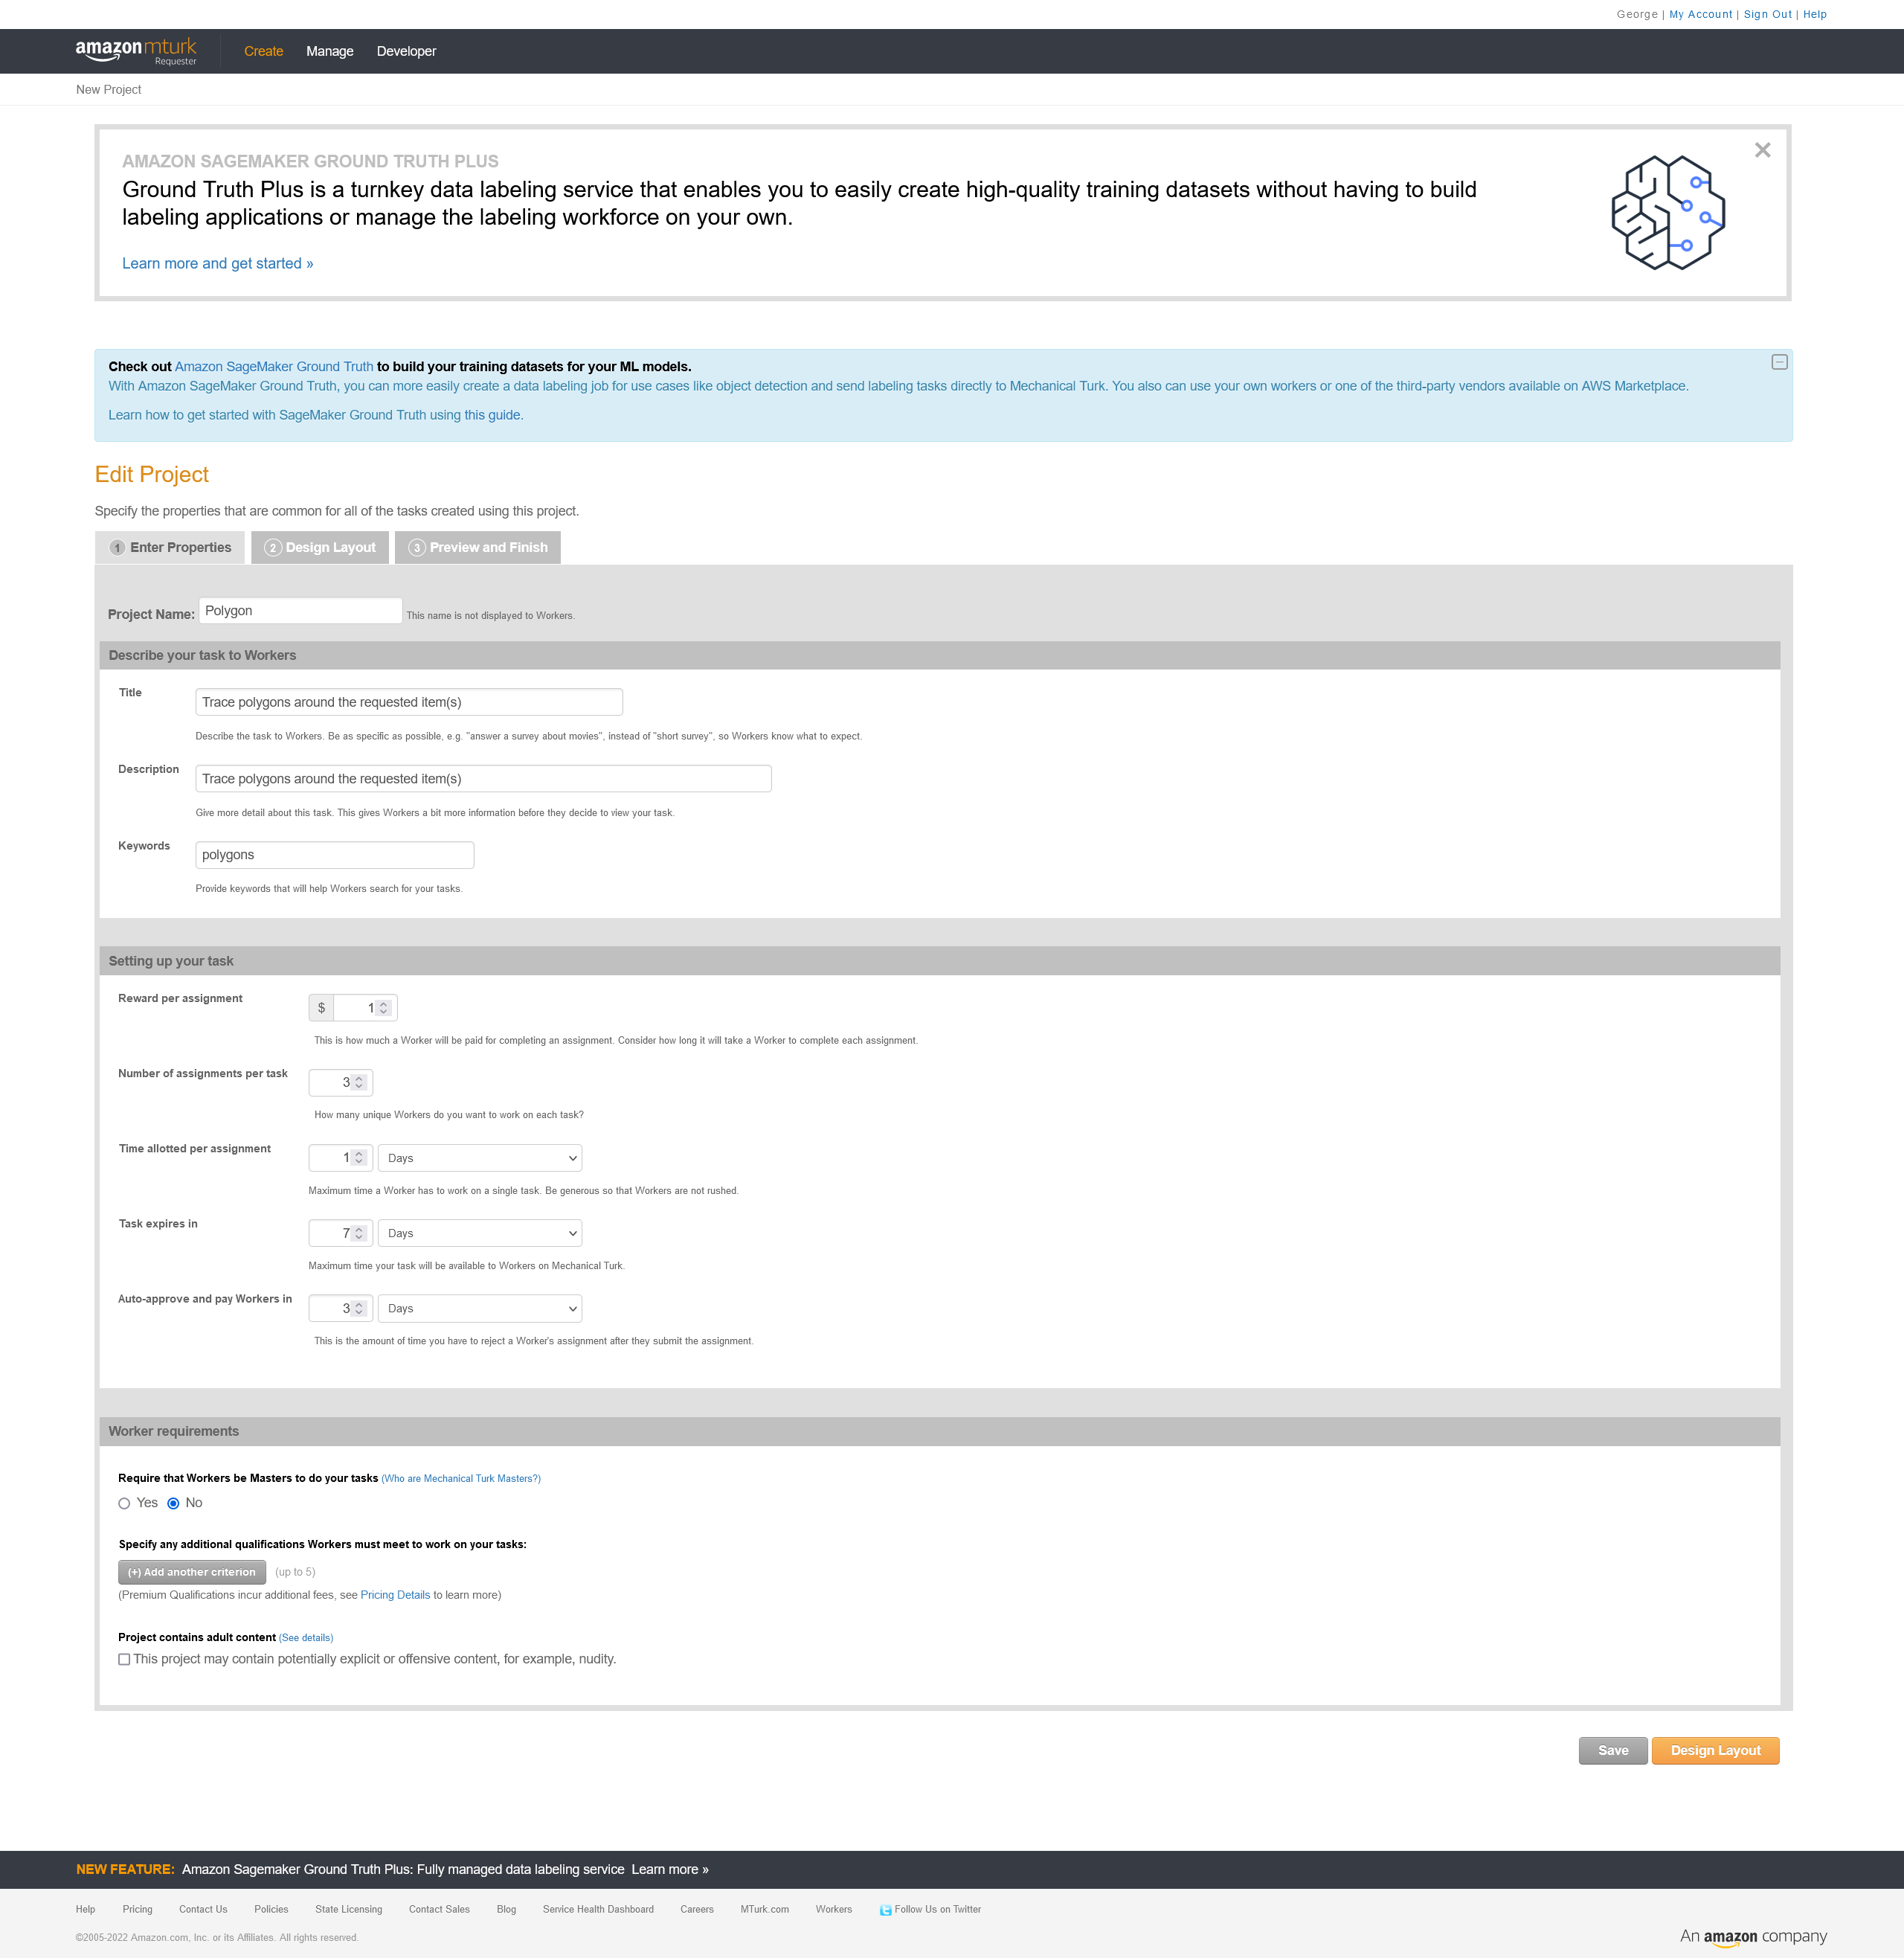
\includegraphics[width=0.9\linewidth]{imgs/mturk/properties.png}
    \caption{任务属性}
    \label{fig:properties}
\end{figure}

\newpage

\begin{figure}[h!]
    \centering
    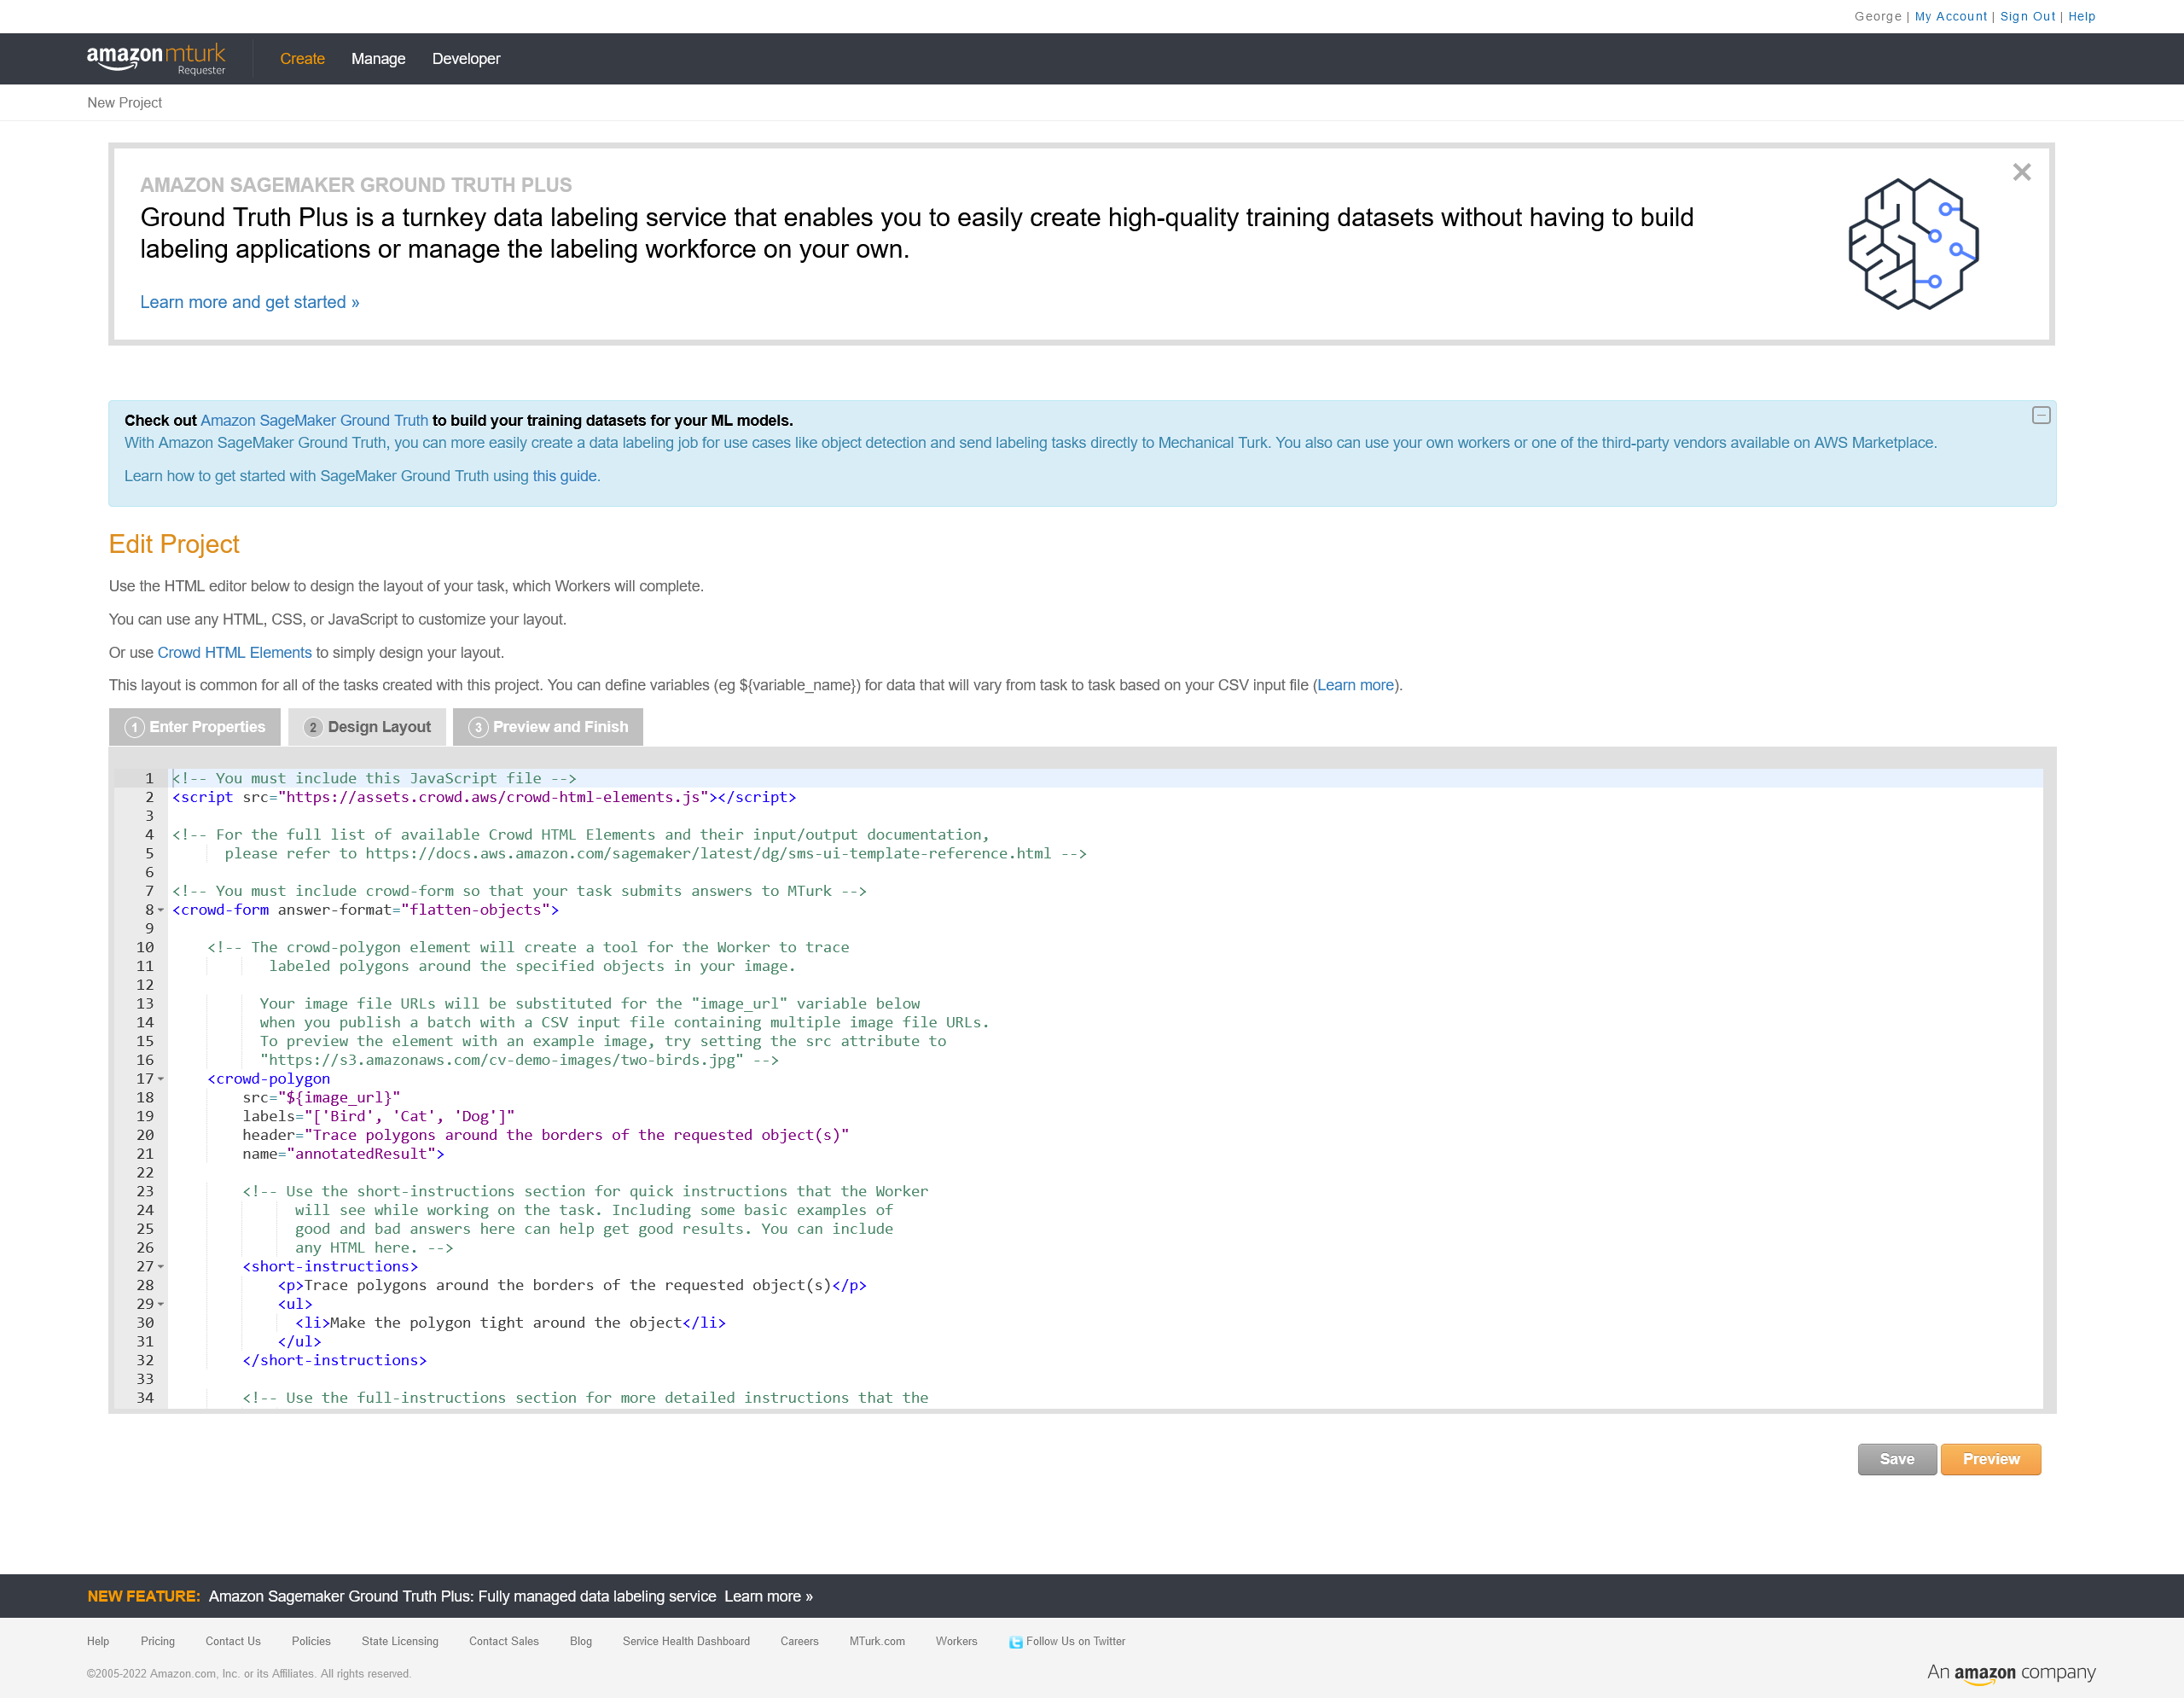
\includegraphics[width=0.7\linewidth]{imgs/mturk/layout.png}
    \caption{任务格式}
    \label{fig:layout}
\end{figure}

\begin{figure}[h!]
    \centering
    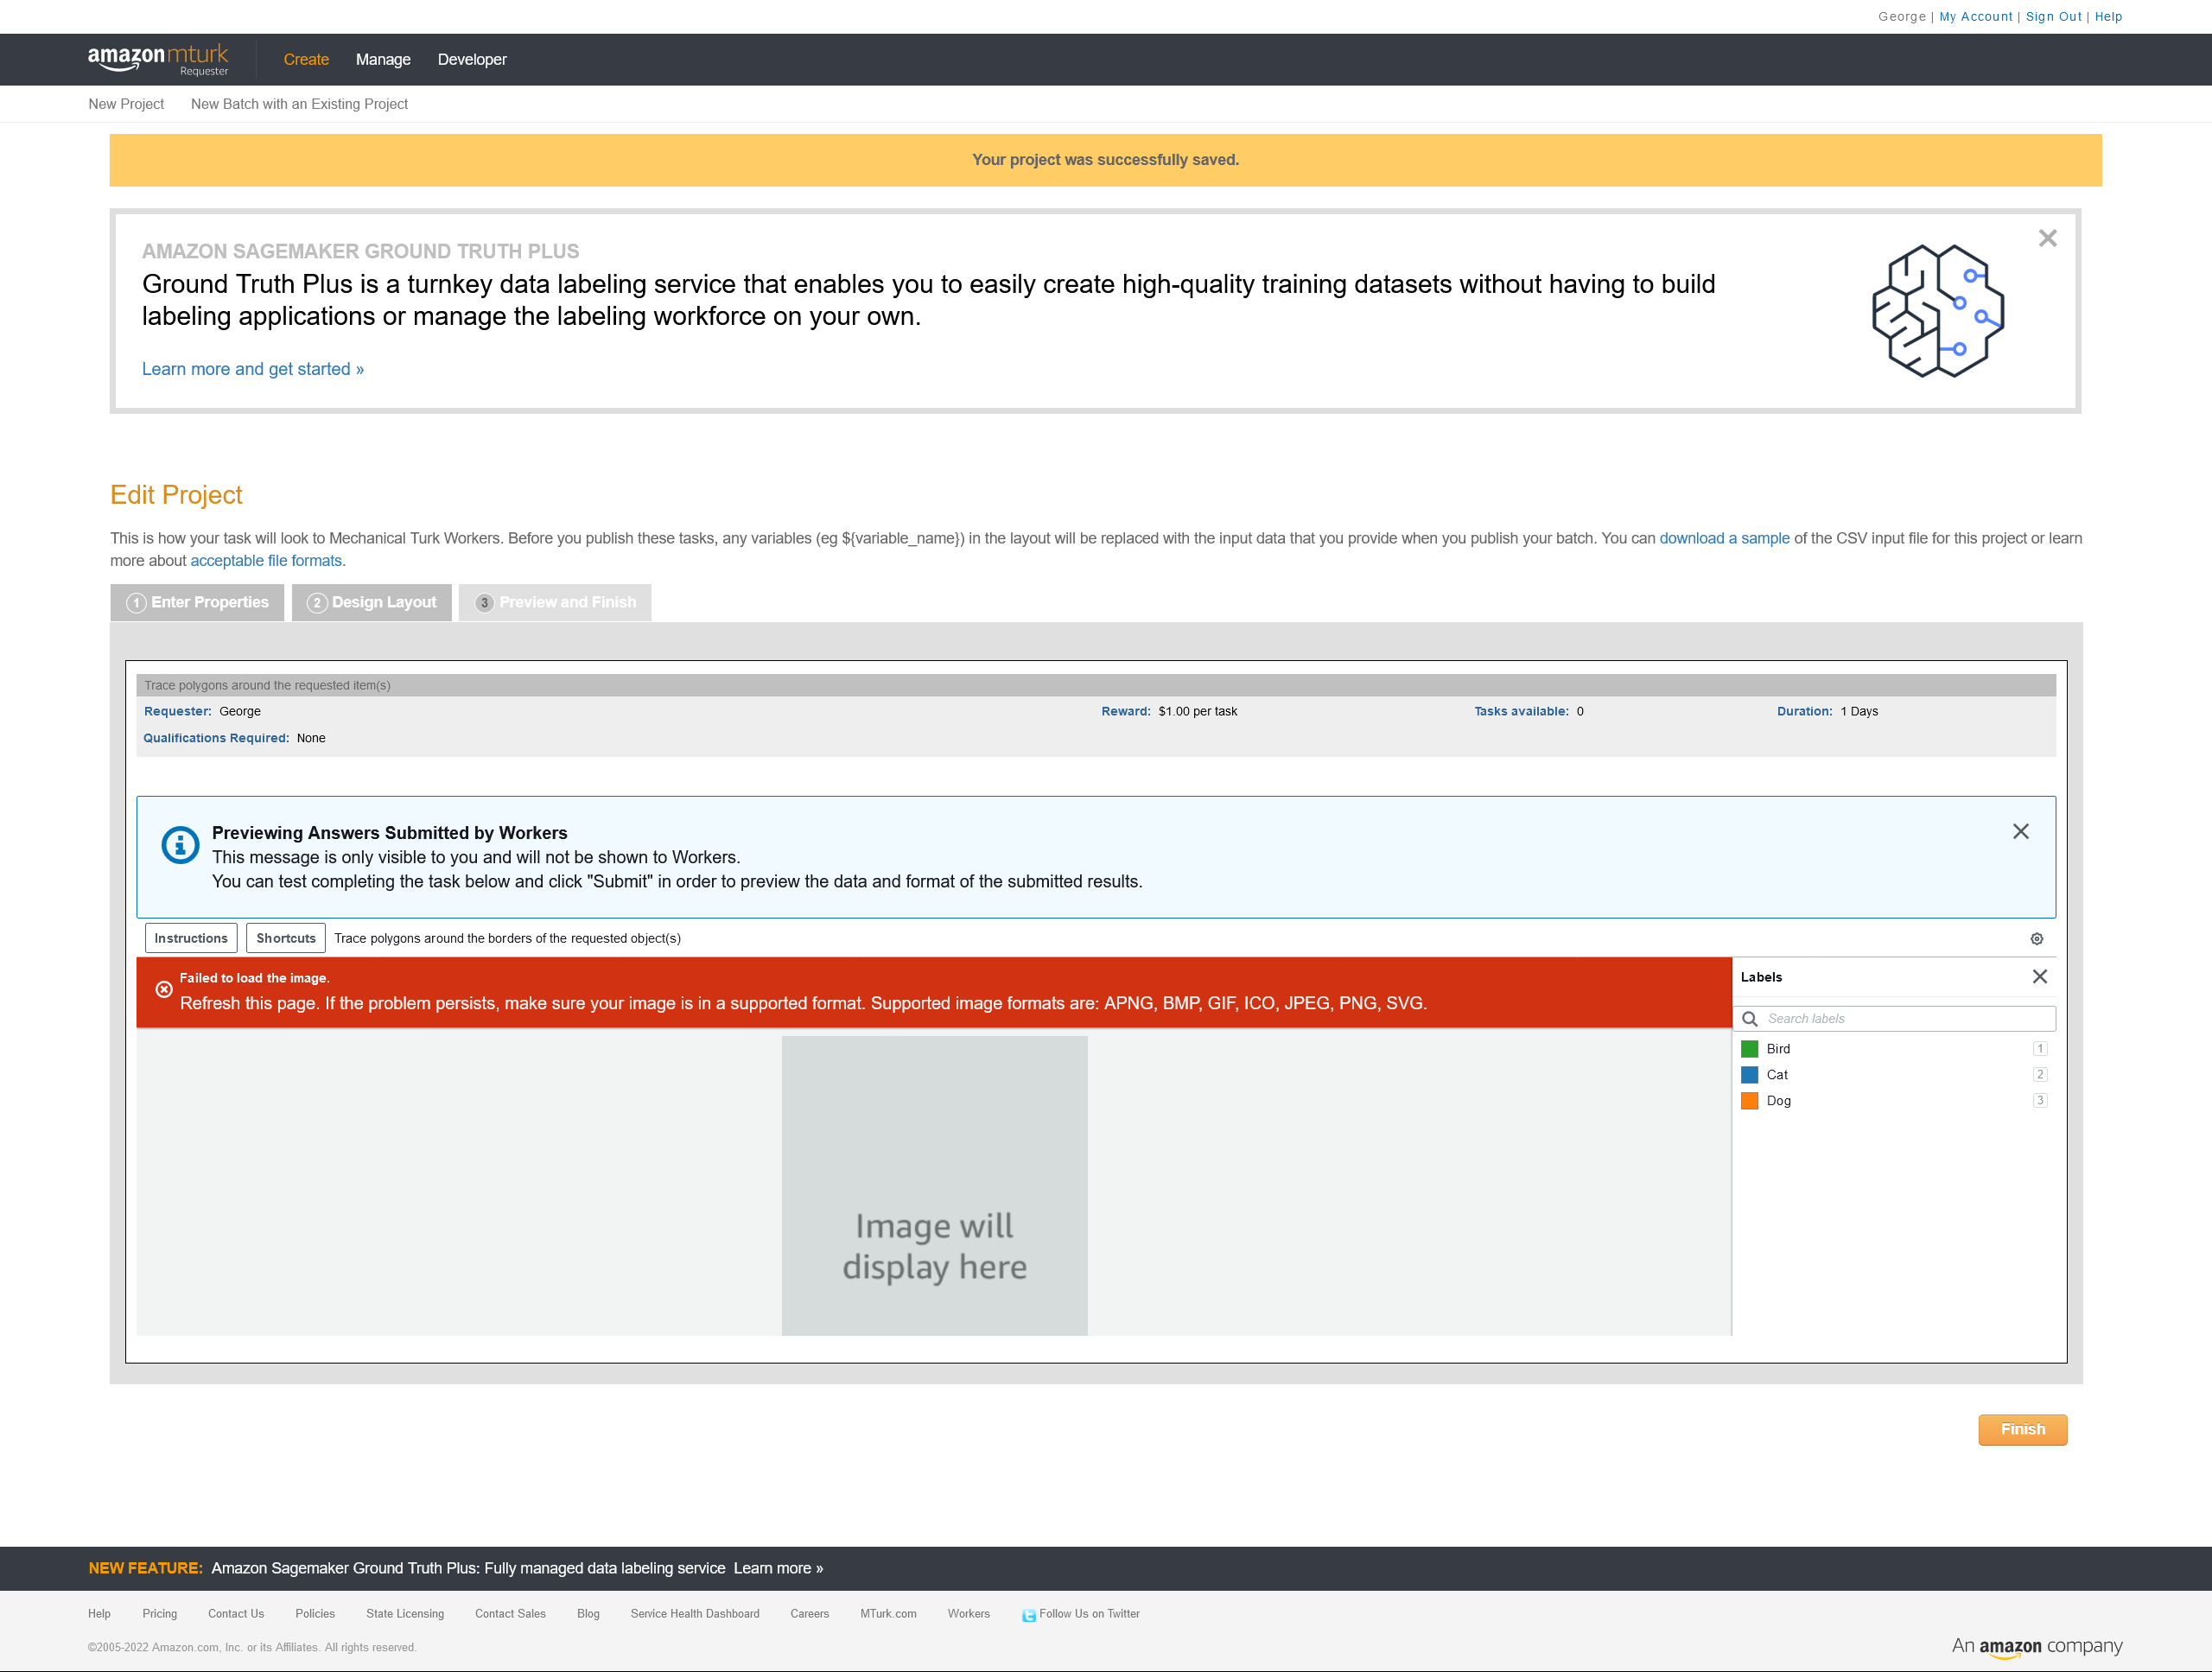
\includegraphics[width=0.7\linewidth]{imgs/mturk/preview.png}
    \caption{任务预览}
    \label{fig:preview}
\end{figure}

\newpage

\begin{figure}[h!]
    \centering
    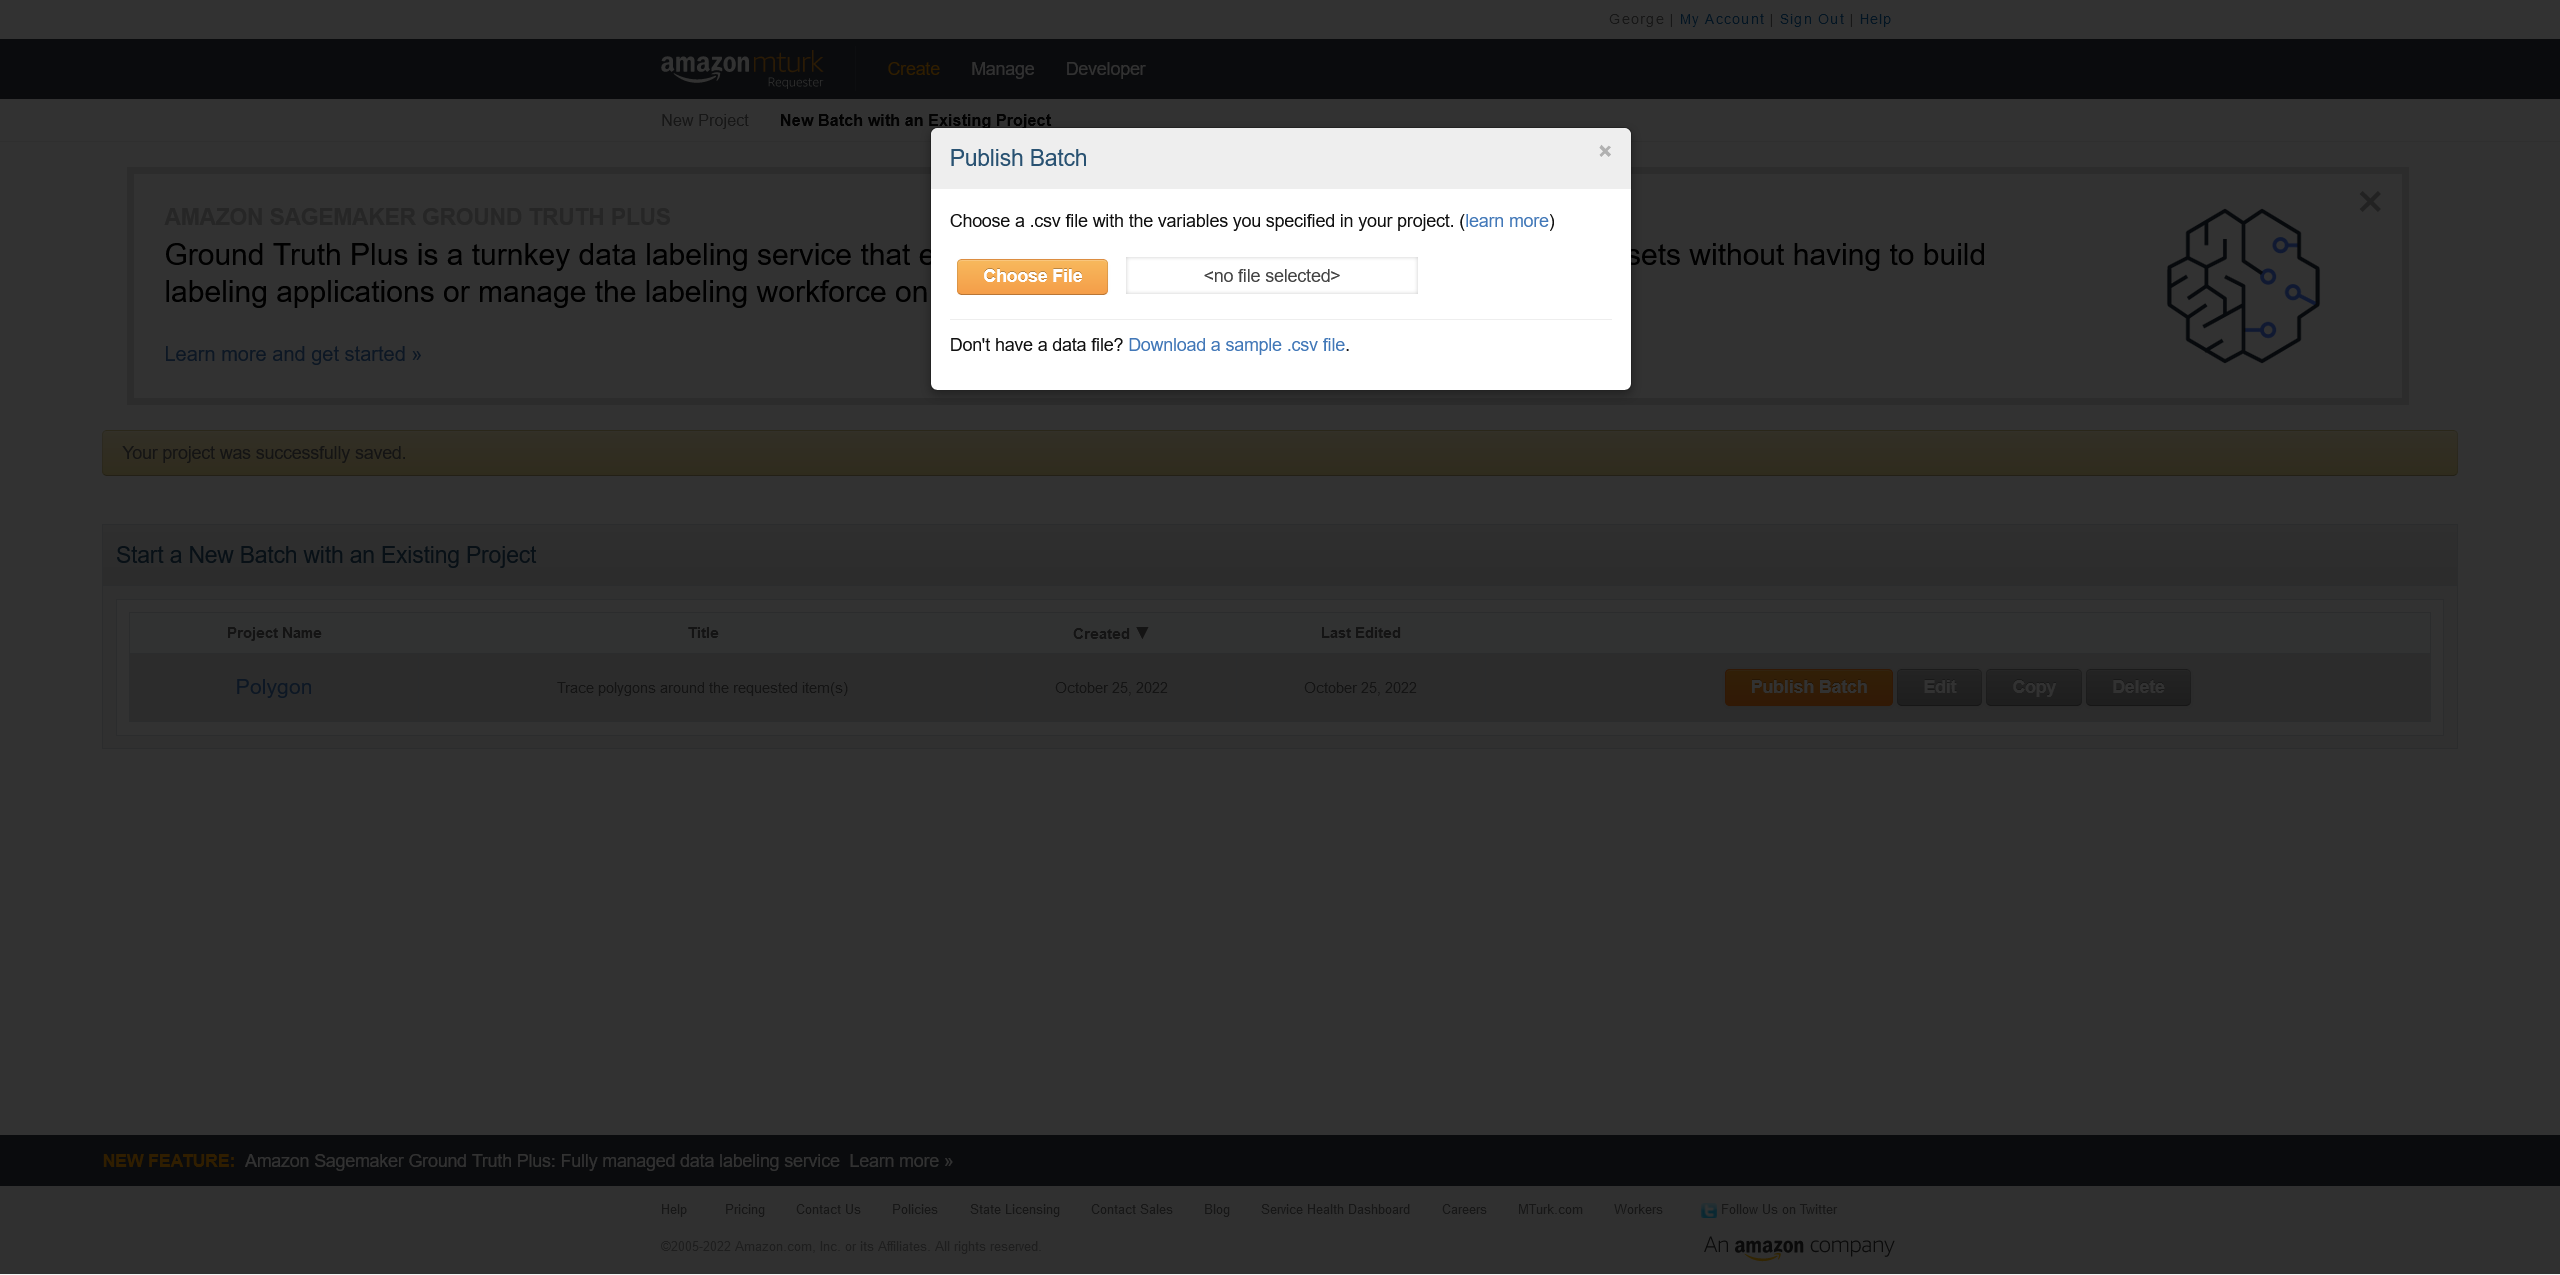
\includegraphics[width=\linewidth]{imgs/mturk/publish.png}
    \caption{任务发布}
    \label{fig:publish}
\end{figure}